\documentclass[a4paper,12pt,reqno]{amsart}
\usepackage{M67tds}

% pour voir les solutions il faut enlever le commentaire de la ligne suivante
\solutionstrue

\newcommand{\cC}{\mathcal C}
\newcommand{\cD}{\mathcal D}
\newcommand{\cE}{\mathcal E}

\begin{document}

% ==================================
\hautdepage{
  \ifsolutions{Solutions de l'interrogation}\else{Interrogation}\fi\par\normalfont\normalsize
  1 avril 2019\\{[ durée: 1 heure ]}\par
}
% ==================================
\sisujet{
  \tikz[baseline=(e.base)]{\NoAutoSpacing\node(e){!};\draw[red,ultra thick,line join=round,yshift=-.15ex](90:1em)--(210:1em)--(330:1em)--cycle;}
  \textbf{Documents autorisés :}\textit{Une feuille A4 recto-verso écrite à la main.}

  \vspace{17mm}
  %\tsvp
}


%-----------------------------------
\begin{exo} (Puissance d'un point par rapport à un cercle)

  Soit $\cC$ un cercle de centre $O$ et de rayon $R$. Soient $M$ un point quelconque à distance $d=OM$ du centre, et $\cD$ une droite passant par $M$ et coupant le cercle en deux points $A$ et $B$ non nécessairement distincts.
  \begin{enumerate}
    \item Donner le signe du produit $\overline{AM}\cdot\overline{BM}$ des longueurs algébriques $\overline{AM}$ et $\overline{BM}$ en fonction de $M$.
    \item On suppose $M$ intérieur au cercle $\cC$. Montrer que le produit $\overline{AM}\cdot\overline{BM}$ est indépendant de la droite $\cD=(AB)$.
    \item Exprimer ce produit en fonction du rayon $R$ et de la distance $d=OM$.
    \item Montrer que les résultats des deux questions précédentes sont encore vrais pour tout point $M$ du plan\footnote{Non nécessairement intérieur au cercle $\cC$.} et toute droite $\cD$ intersectant le cercle.
  \end{enumerate}
  On appelle \emph{puissance de $M$ par rapport au cercle $\cC$} le scalaire ainsi défini, noté $\pi_{\cC}(M)$.
\end{exo}

\begin{solution}

  \begin{enumerate}
    \item Si $A \neq B$ alors $[AB]$ est l'intersection du disque fermé de centre $O$ et de rayon $R$ et de la droite $\cD$. Ainsi, si $M$ est à l'extérieur du cercle, il ne peut être entre $A$ et $B$, par convexité du disque. Les longueurs algébriques $\overline{AM}$ et $\overline{BM}$ sont donc de même signe, et $\overline{AM}\cdot\overline{BM}$ est positif. Si $M$ est à l'intérieur du cercle, $M$ est alors entre $A$ et $B$, et $\overline{AM}\cdot\overline{BM}$ est négatif. Enfin, si $M$ est sur le cercle, le produit est nul.
    \item Si $M$ est intérieur au cercle, on a $\overline{AM}\cdot\overline{BM}=-{AM}\cdot{BM}$. Soient $\cD$ et $\cD'$ deux droites distinctes passant par $M$ coupant respectivement $\cC$ en $A \neq B$, et en $A' \neq B'$ (une droite passant par $M$ intérieur au cercle le coupe en deux points distincts). On a nécessairement $A \neq A'$ et $B \neq B'$ du fait que $\cD\neq\cD'$.
    \sidebyside{.7}{
      Les deux angles inscrits $\widehat{ABA'}$ et $\widehat{A'B'A}$ interceptent le même arc $\wideparen{AA'}$\footnotemark, donc sont égaux. Les deux angles $\widehat{AMB'}$ et $\widehat{A'MB}$ opposés par le sommet sont égaux. Les triangles $AMB'$ et $A'MB$ sont donc semblables, et on a en particulier $\frac{MA}{MA'}=\frac{MB'}{MB}$. D'où $\overline{AM}\cdot\overline{BM}=-{AM}\cdot{BM}=-{A'M}\cdot{B'M}=\overline{A'M}\cdot\overline{B'M}$.
    }{
      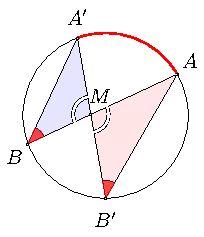
\includegraphics[width=4cm,valign=t,Trim=-3mm 17mm]{M67_2018-19_CC_exo1b.pdf}
    }
    \footnotetext{Pour justifier ce fait, on peut remarquer que $B$ et $M$ (resp. $B'$ et $M$) sont du même côté de $(AA')$, de sorte que $B$ et $B'$ sont du même côté de $(AA')$.}
    \item
    \sidebyside{.7}{
      Puisque ce produit est indépendant de la droite $\cD$ passant par $M$ considérons la droite $(OM)$ si $M \neq O$ ou n'importe quelle droite si $M=O$, de sorte que $A$ et $B$ sont antipodaux. Alors, puisque $M$ est entre $A$ et $B$, on a $\overline{AM}\cdot\overline{BM}=-AM \cdot BM=-(R-OM)(R+OM)=d^2-R^2$.
    }{
      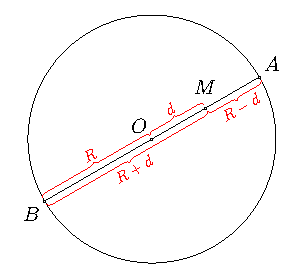
\includegraphics[width=4cm,valign=t,Trim=-3mm 8mm]{M67_2018-19_CC_exo1c.pdf}
    }
    \item
    Si $M$ est sur le cercle, alors pour toute droite $\cD$ passant par $M$ et coupant $\cC$ en $A=M$ et $B$ on a $\overline{AM}\cdot\overline{BM}=0=d^2-R^2$ puisque dans ce cas $d=R$.
    \sidebyside{.7}{\vspace{7mm}
      Si $M$ est à l'extérieur du cercle et si $\cD$ passe par $M$ et coupe $\cC$ en $A$ et $B$, pas forcément distincts, tels que $A\in [M,B]$, alors $\overline{AM}\cdot\overline{BM}=AM \cdot BM$. Soit $\cD'$ une autre droite passant par $M$ et coupant $\cC$ en $A'$ et $B'$ avec $A'\in [M,B']$. Montrons que $AM \cdot BM=A'M \cdot B'M$. Les angles inscrits $\widehat{MBA'}$ et $\widehat{MB'A}$ interceptent le même arc $\wideparen{AA'}$, donc sont égaux. Les triangles $MA'B$ et $MAB'$ (qui partagent leur angle en $M$) sont donc semblables, et $\frac{A'M}{AM}=\frac{BM}{B'M}$.
    }{
      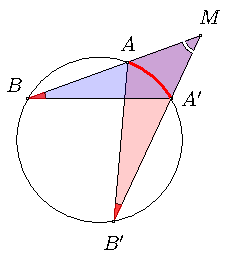
\includegraphics[width=4cm,valign=t,Trim=-3mm 14mm]{M67_2018-19_CC_exo1d1.pdf}\\
      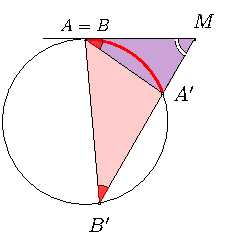
\includegraphics[width=4cm,valign=t,Trim=-3mm -11mm]{M67_2018-19_CC_exo1d2.pdf}
    }\vspace{-4mm}
    \sidebyside{.7}{
      Pour finir, si $\cD=(OM)$, alors $M,A,O,B$ sont alignés dans cet ordre et $AM\cdot BM=(d-R)(d+R)=d^2-R^2$.
    }{
      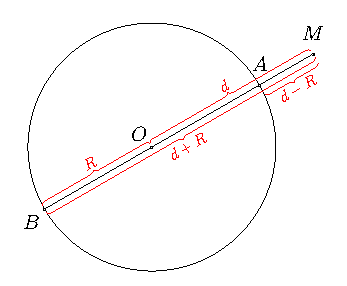
\includegraphics[width=4cm,valign=t,Trim=-3mm 17mm]{M67_2018-19_CC_exo1d3.pdf}
    }
  \end{enumerate}
\end{solution}

\sisujet{\bigskip}
\sisolutions{\newpage}

%-----------------------------------
\begin{exo} (Kangourou 2016)

  \sidebyside{.56}{
    Sur la figure ci-contre la droite $(XP)$ est tangente en $P$ au cercle de centre $O$ et de diamètre $[MN]$. Si les longueurs des arcs $\wideparen{MP}$ et $\wideparen{NP}$ sont respectivement $20$ et $16$, combien vaut l'angle $\widehat{OXP}$ ?
  }{
    \raisebox{-17mm}[0pt][0pt]{\includegraphics[width=7cm]{img_kangourou2016}}
  }
\end{exo}

\begin{solution}

  Comme le demi périmètre du cercle est $36$, alors $\widehat{POX}=\frac{16}{36}180°=80°$. Et comme $OP\perp PX$, car $PX$ tangente, on a $\widehat{OXP}=90°-\widehat{POX}=10°$.

  Une autre solution possible est de dire que $\widehat{OXP}=\frac12(\wideparen{MP} - \wideparen{PN})= \frac12\big(\frac{20}{36}-\frac{16}{36}\big)180°= 10°$.
\end{solution}

\end{document}
